\section*{Les maquettes}
\addcontentsline{ptc}{section}{Les maquettes}
\label{sec:maquettes}

Voici les différentes maquettes du site :

\begin{figure}[!h]
    \centering
    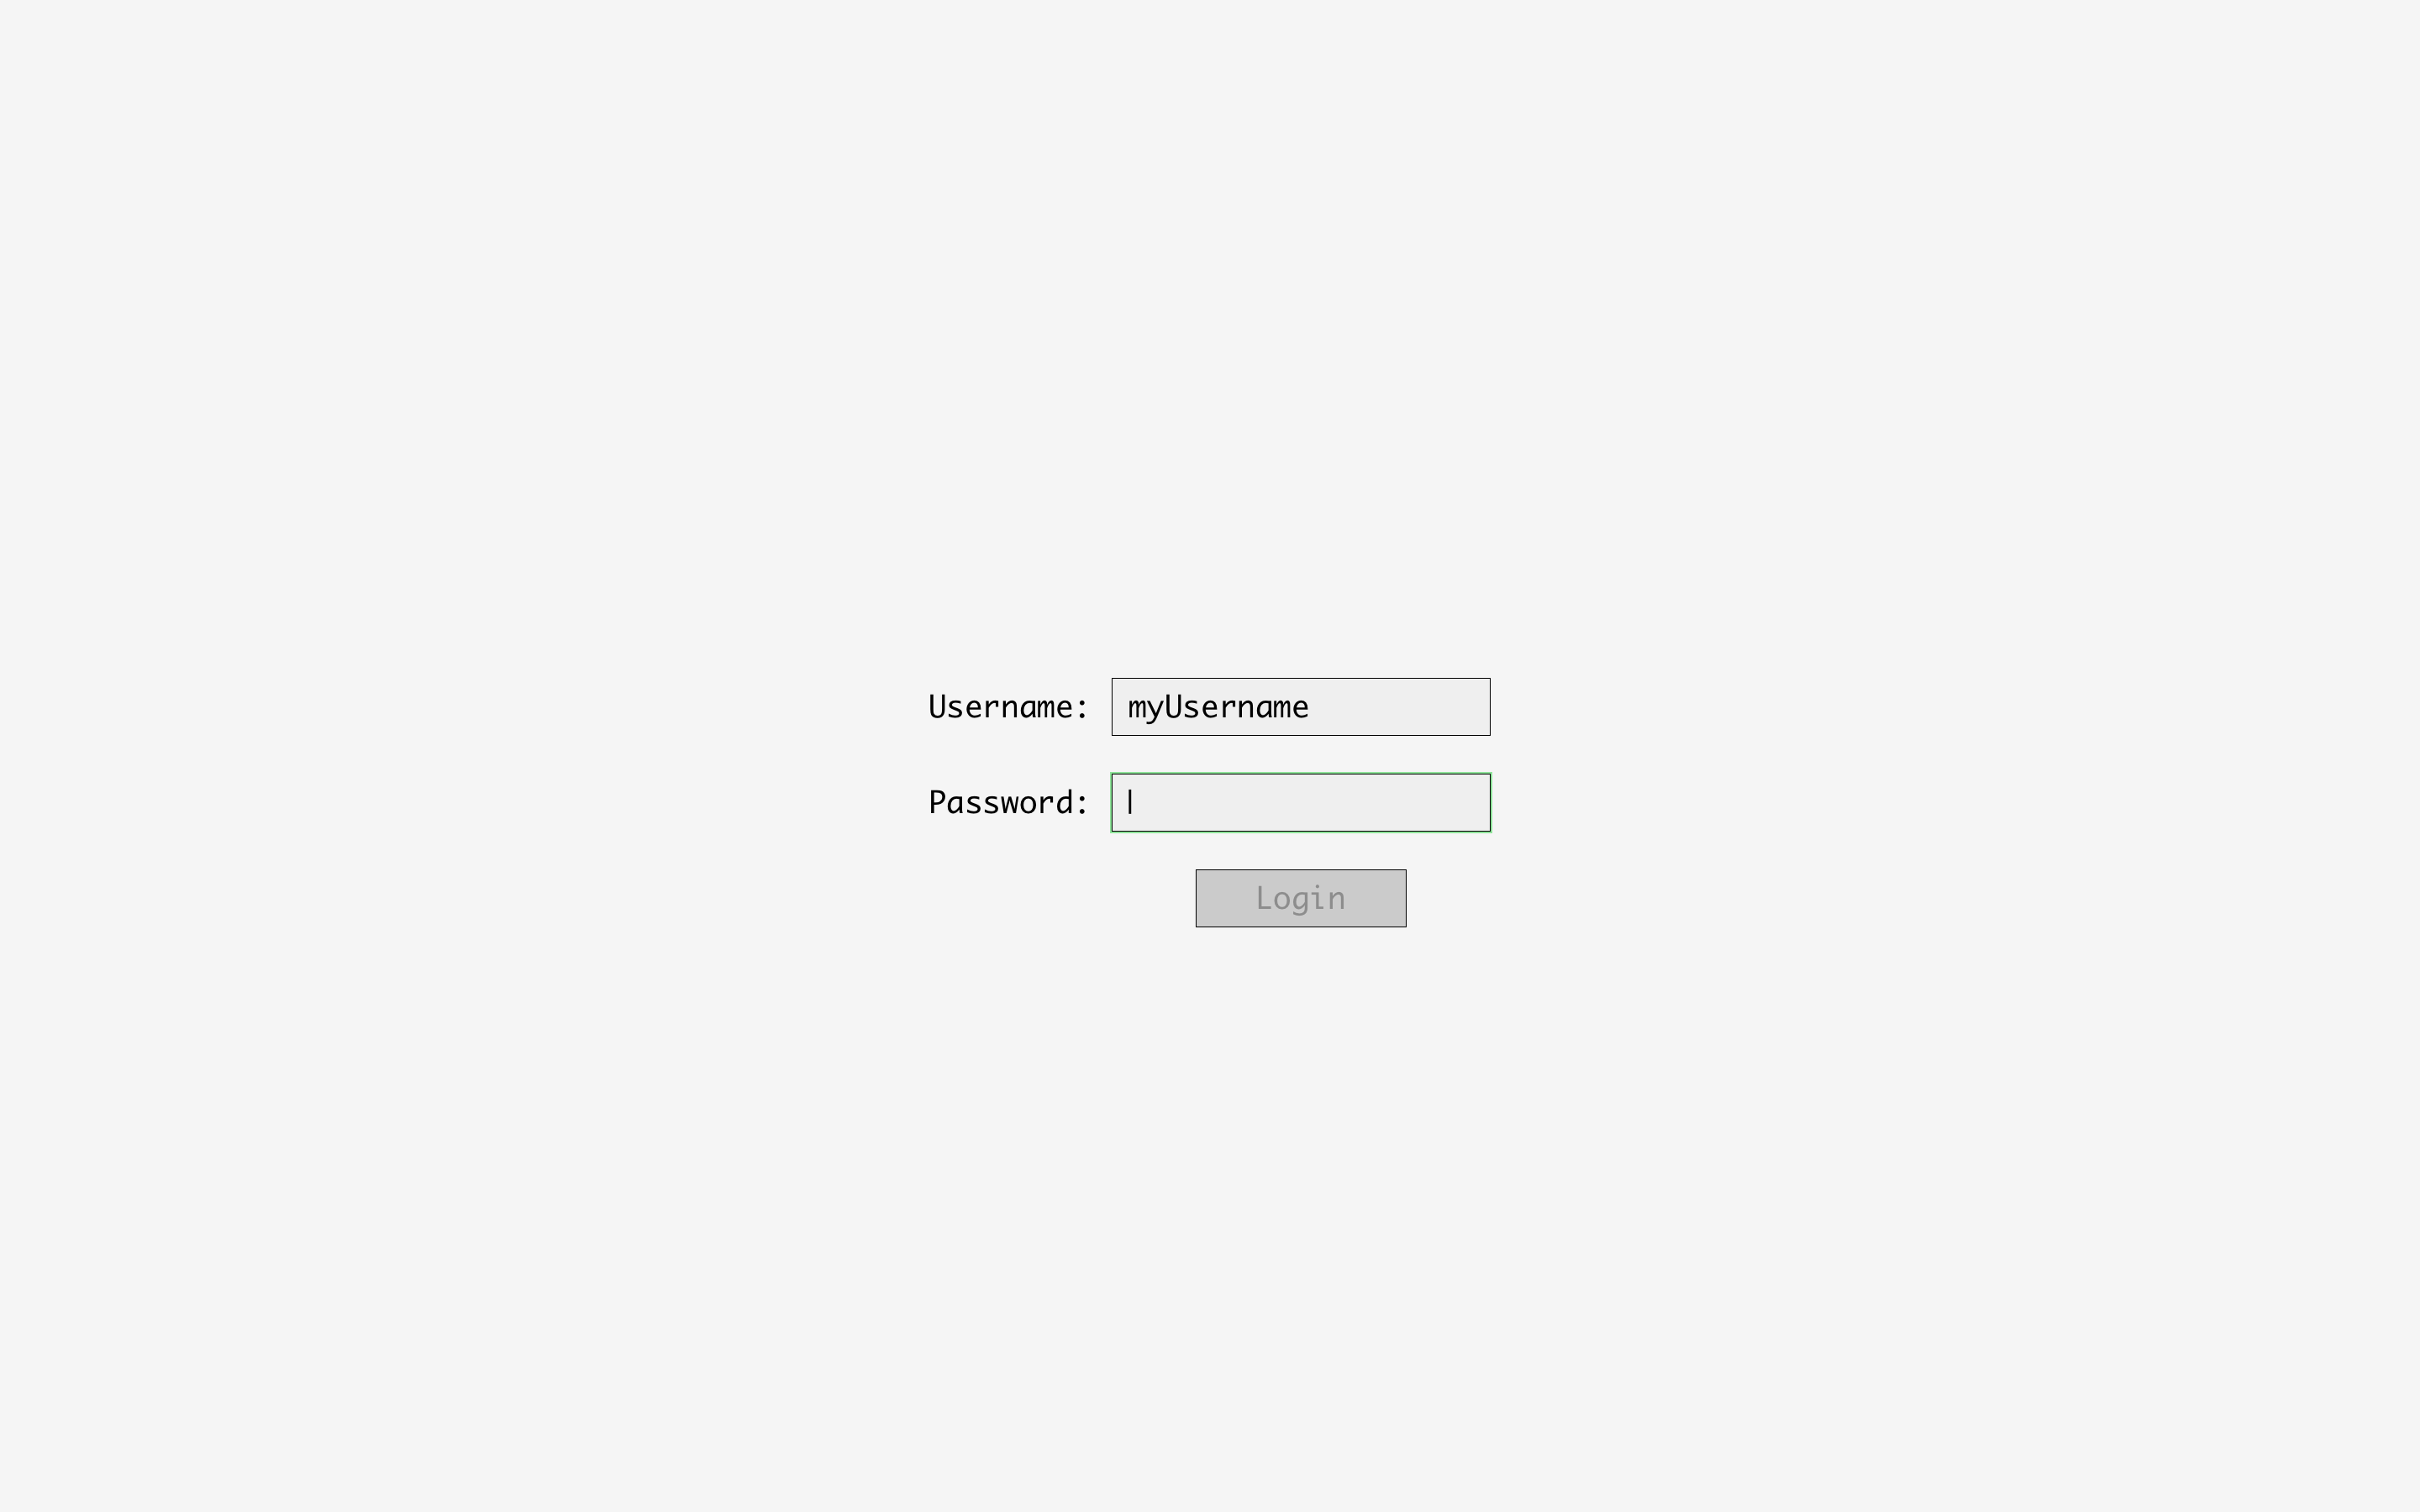
\includegraphics[scale=0.14]{textures/images/annexes/maquettes/1-Login.png}
    \caption{La page d'accueil}
\end{figure}
\begin{figure}[!h]
    \centering
    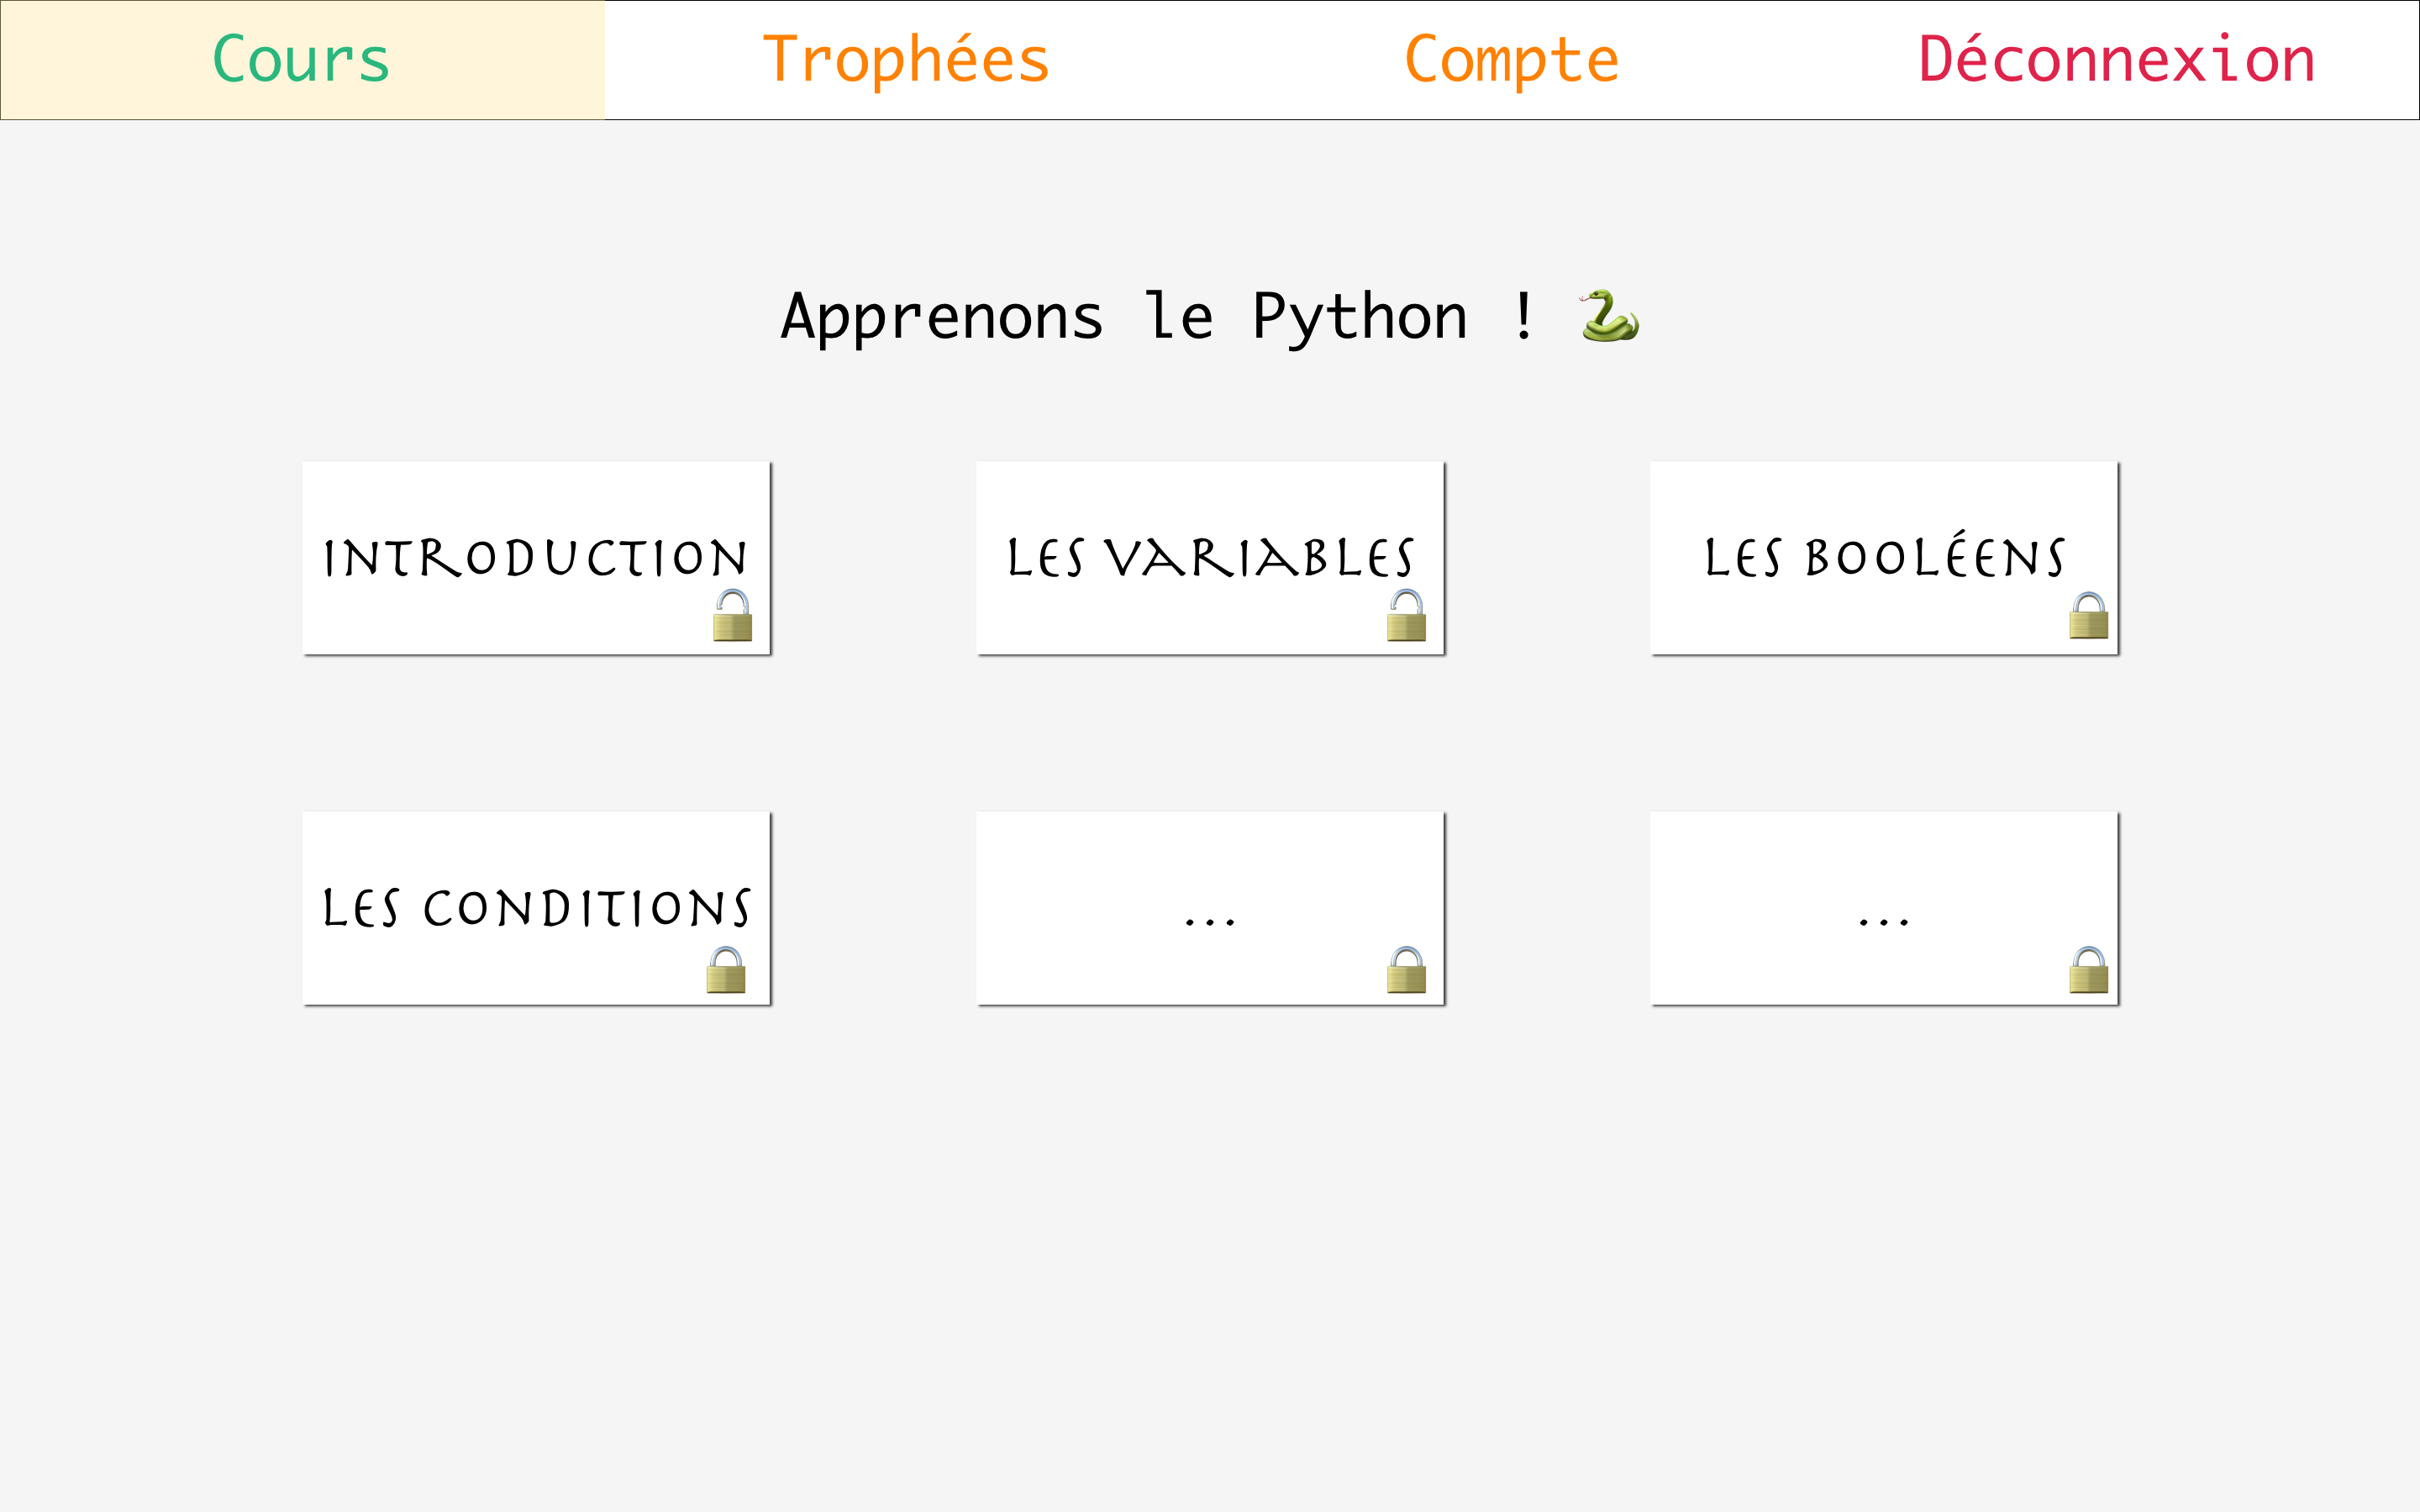
\includegraphics[scale=0.14]{textures/images/annexes/maquettes/21-Sommaire.png}
    \caption{La page de cours}
\end{figure}

\newpage

\begin{figure}[!h]
    \centering
    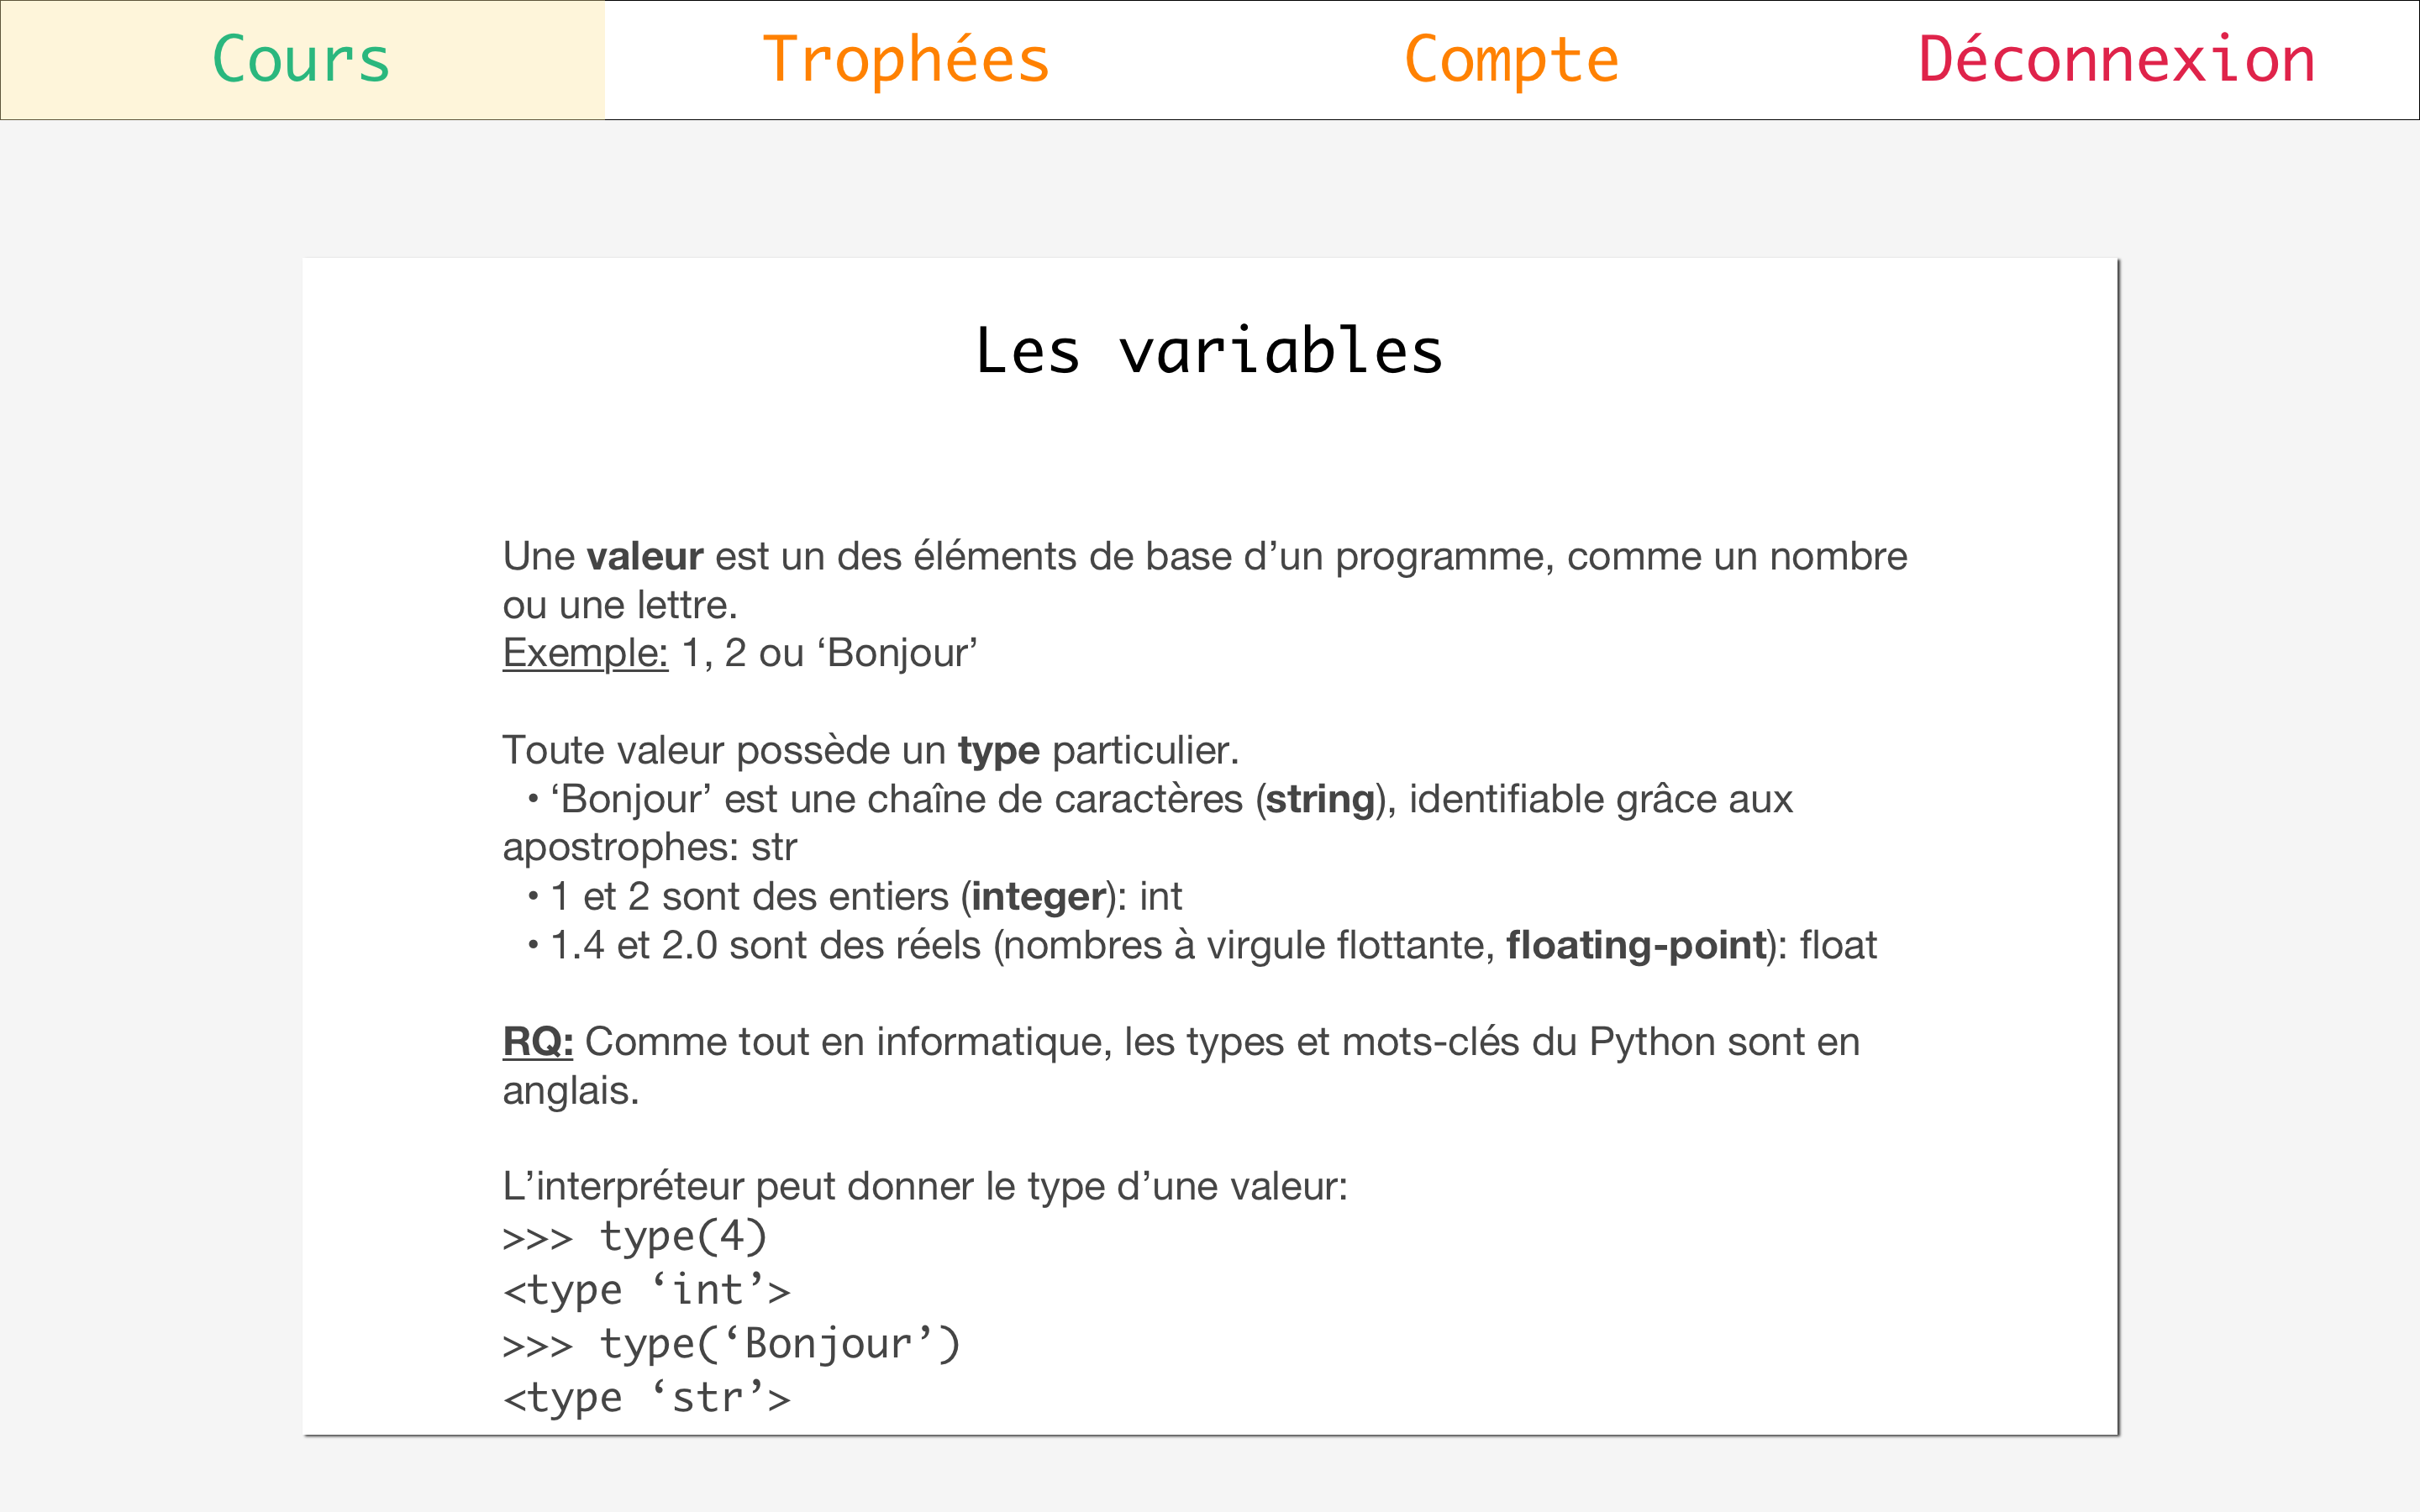
\includegraphics[scale=0.14]{textures/images/annexes/maquettes/22-Cours.png}
    \caption{L'aperçu d'un chapitre}
\end{figure}
\begin{figure}[!h]
    \centering
    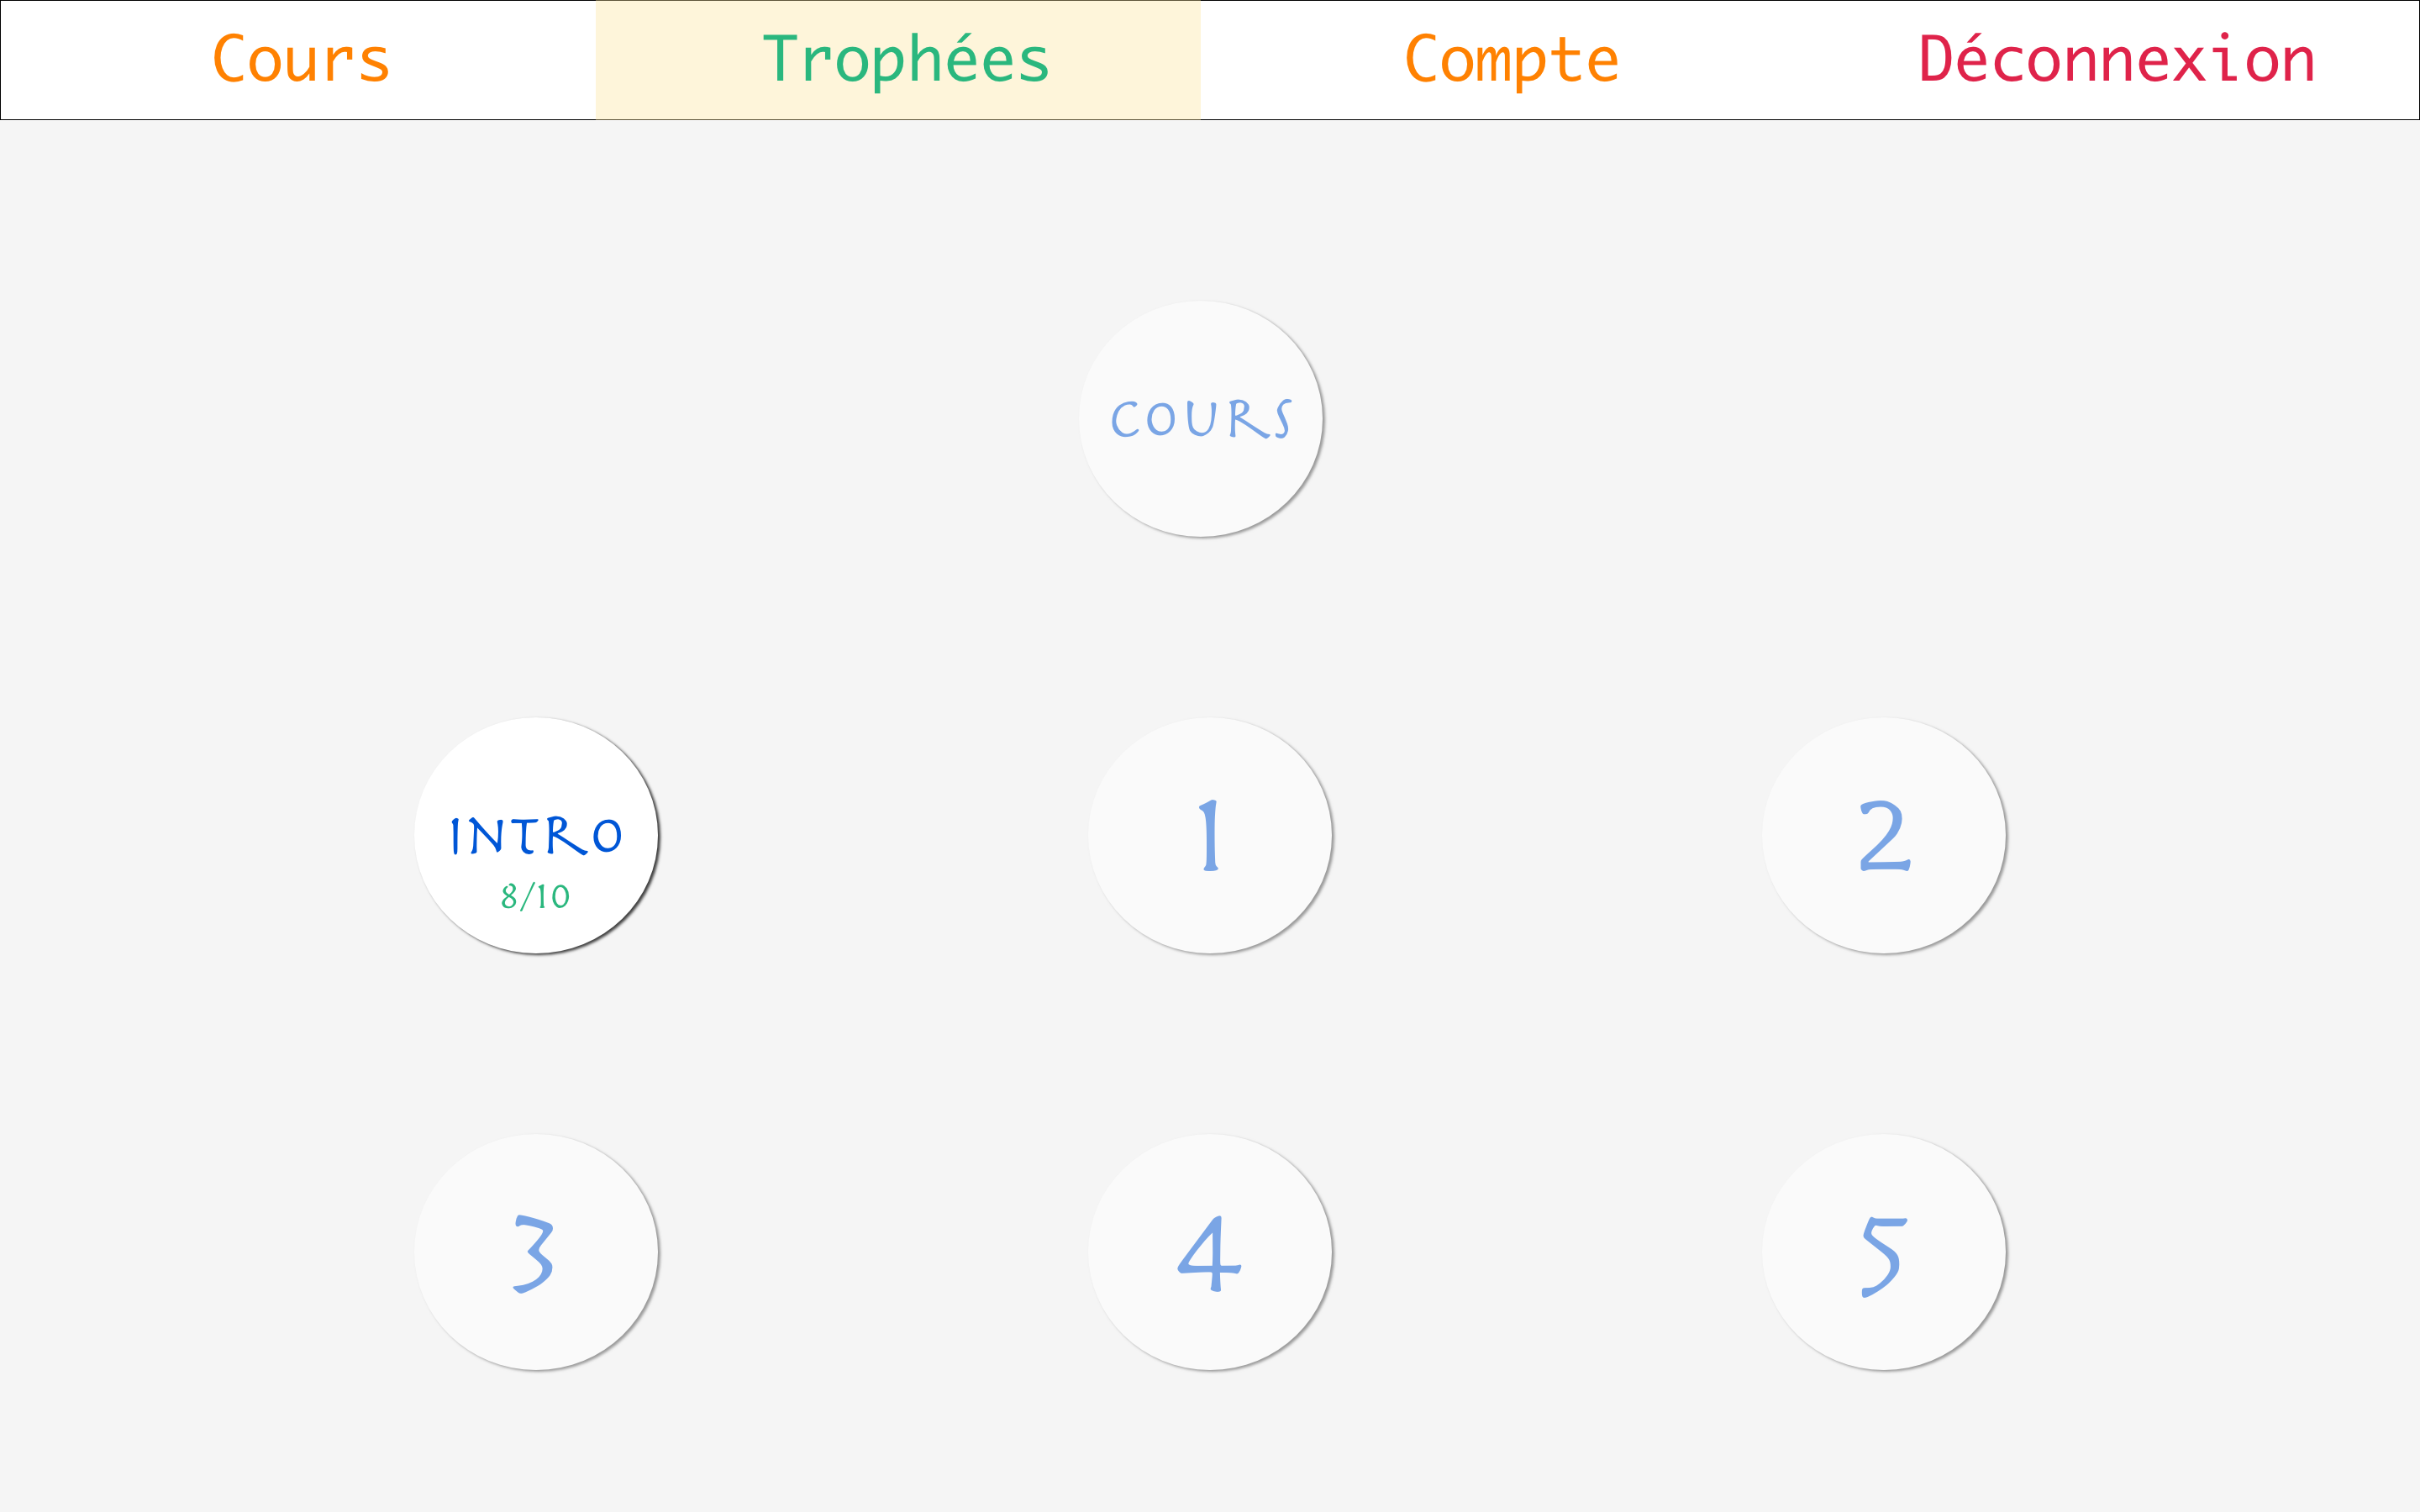
\includegraphics[scale=0.14]{textures/images/annexes/maquettes/3-Trophees.png}
    \caption{La page des trophées}
\end{figure}

\newpage

\begin{figure}[!h]
    \centering
    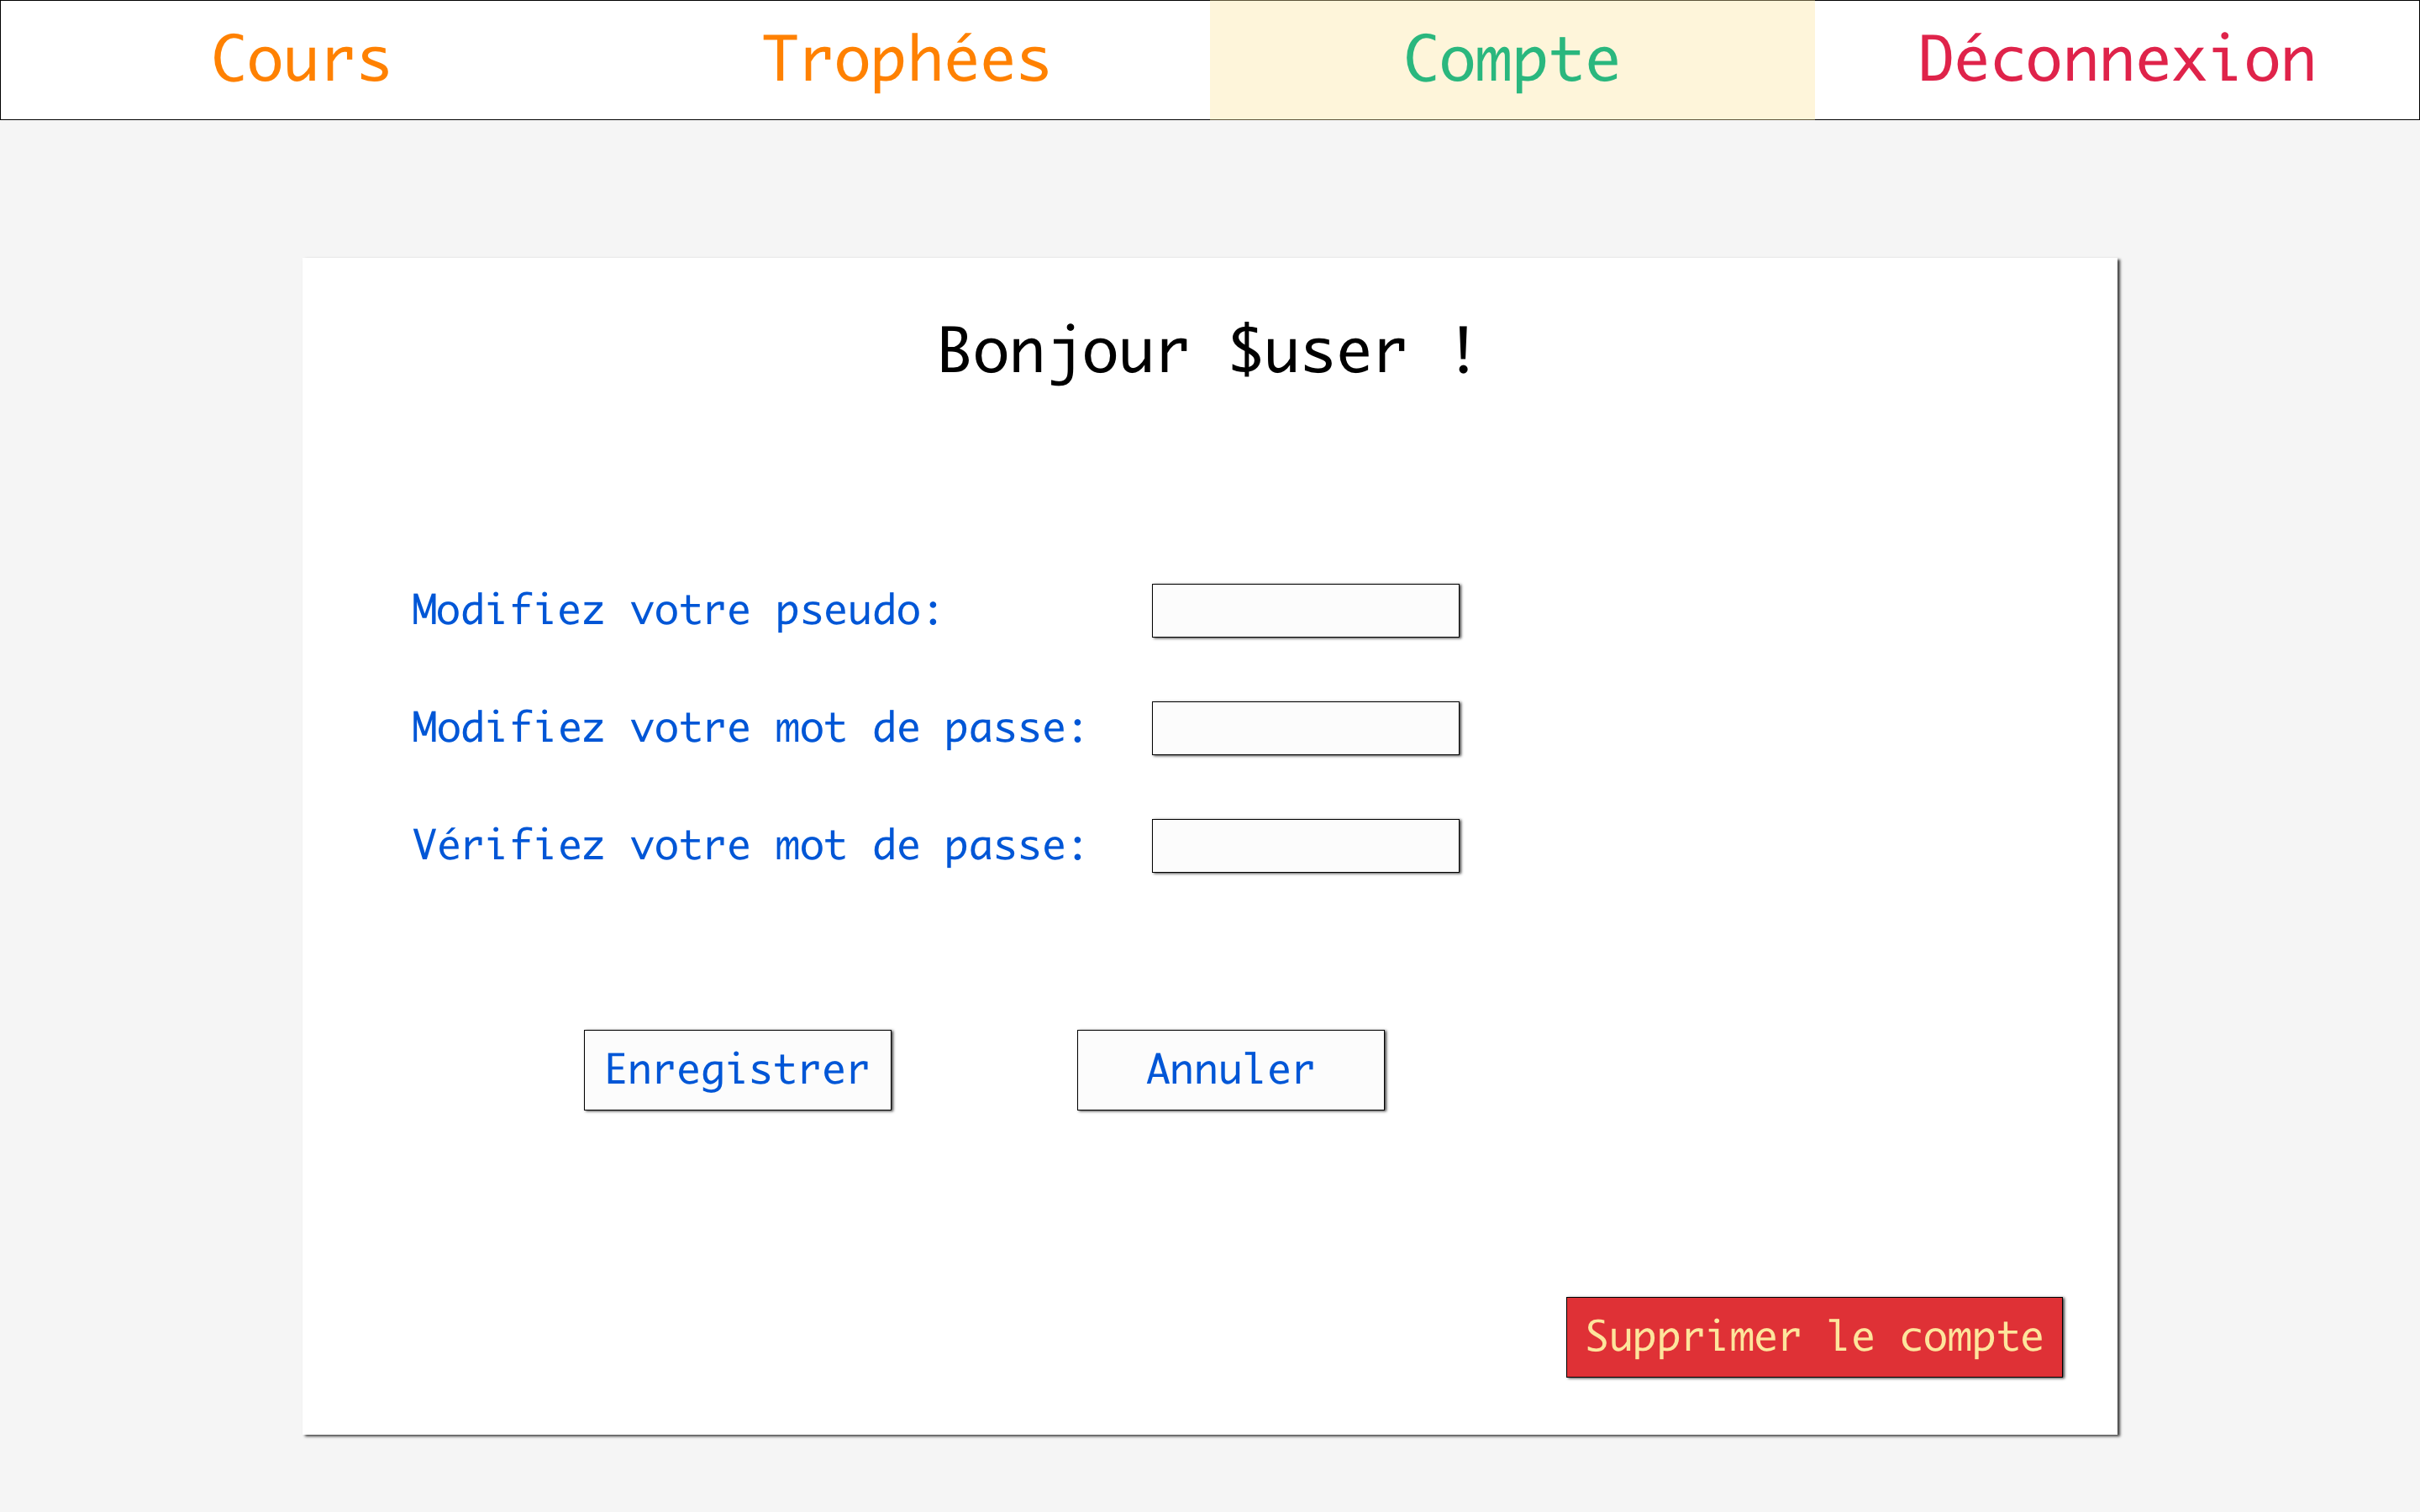
\includegraphics[scale=0.14]{textures/images/annexes/maquettes/4-Compte.png}
    \caption{La page du compte}
\end{figure}